\documentclass[12pt]{article}
\usepackage[margin=2.5cm]{geometry}
\usepackage{enumerate}
\usepackage{amsfonts}
\usepackage{amsmath}
\usepackage{fancyhdr}
\usepackage{amsmath}
\usepackage{amssymb}
\usepackage{amsthm}
\usepackage{mdframed}
\usepackage{graphicx}
\usepackage{subcaption}
\usepackage{adjustbox}
\usepackage{listings}
\usepackage{xcolor}
\usepackage{courier}
\usepackage[utf]{kotex}
\usepackage{hyperref}
\usepackage{soul}

\definecolor{codegreen}{rgb}{0,0.6,0}
\definecolor{codegray}{rgb}{0.5,0.5,0.5}
\definecolor{codepurple}{rgb}{0.58,0,0.82}
\definecolor{backcolour}{rgb}{0.95,0.95,0.92}

\lstdefinestyle{mystyle}{
    backgroundcolor=\color{backcolour},
    commentstyle=\color{codegreen},
    keywordstyle=\color{magenta},
    numberstyle=\tiny\color{codegray},
    stringstyle=\color{codepurple},
    basicstyle=\ttfamily\footnotesize,
    breakatwhitespace=false,
    breaklines=true,
    captionpos=b,
    keepspaces=true,
    numbers=left,
    numbersep=5pt,
    showspaces=false,
    showstringspaces=false,
    showtabs=false,
    tabsize=1
}

\lstset{style=mystyle}

\pagestyle{fancy}
\renewcommand{\headrulewidth}{0.4pt}
\lhead{CSC 369}
\rhead{Midterm 3 Notes}

\begin{document}
\title{CSC 369 Midterm 4 Notes}

\section{Critical Section}

\begin{itemize}
    \item Is a piece of code that accesses a \textit{shared} resource,
    \ul{usually a variable or data structure}
\end{itemize}

\section{Thread}

\begin{itemize}
    \item Is a lightweight process that can be managed independently by a schdeduler $^{[4]}$
    \item Improves the application performance using parallelism. (e.g peach)

    \begin{center}
    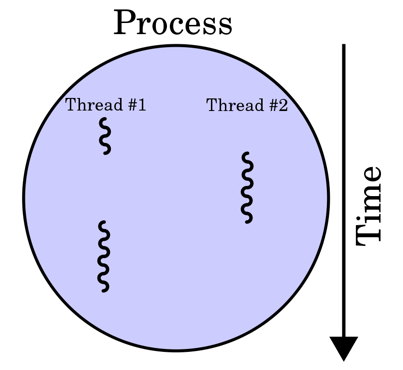
\includegraphics[width=0.4\linewidth]{../../images/midterm_2_solution_1.png}
    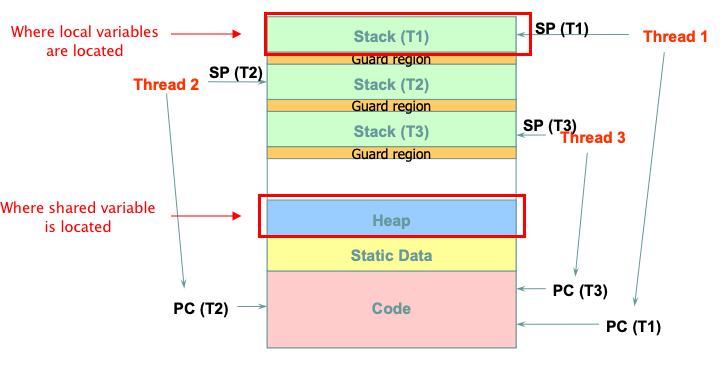
\includegraphics[width=\linewidth]{../../images/midterm_2_solution_2.png}
    \end{center}

    \item A thread is bound to a single process
    \item A process can have multiple threads
    \item Has two types
    \begin{itemize}
        \item \textbf{User-level Threads:}

        \begin{itemize}
            \item Are implemented by users and kernel is not aware of the existence of these threads
            \item Are represented by a program counter(PC), stack, registers and a small process control block
            \item Are small and much faster than kernel level threads
        \end{itemize}
        \item \textbf{Kernel-level Threads:}

        \begin{itemize}
            \item Are handled by the operating system directly
            \item Thread management is done by the kernel
            \item Are slower than user-level threads
        \end{itemize}
    \end{itemize}
\end{itemize}

\section{Thread API}

\begin{itemize}

    \item \texttt{pthread\_create}

    \begin{itemize}
        \item \textbf{syntax:}

        \bigskip
\begin{lstlisting}[language=c]
int pthread_create(pthread_t *thread,
               const pthread_attr_t *attr,
               void * (*start_routine)(void*),
               void * arg)
\end{lstlisting}

        \begin{itemize}
            \item \texttt{thread}

            \begin{itemize}
                \item is a pointer to a structure of type \texttt{pthread\_t}
            \end{itemize}
            \item \texttt{attr}

            \begin{itemize}
                \item is used to specify any attributes this thread might have
                \item is initialized with a separate call \texttt{pthread\_attr\_init()}
                \item set default by passing \texttt{NULL}
            \end{itemize}

            \item \texttt{(start\_routine)}

            \begin{itemize}
                \item means which function this thread should start running in?
                \item setting void pointer \texttt{(void *)} as an argument to function \texttt{start\_routine}
                allows us to pass in \underline{any} type of argument
                \item setting void pointer \texttt{(void *)} as return type allows us to return
                \underline{any} type of result
            \end{itemize}

            \item \texttt{args}

            \begin{itemize}
                \item is where to pass the arguments for the function pointer \texttt((start\_routine))
            \end{itemize}

            \bigskip

            \underline{\textbf{Example}}

            \begin{center}
            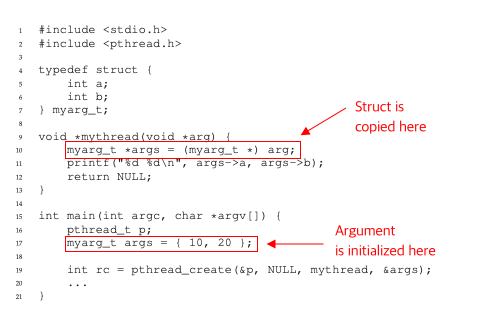
\includegraphics[width=\linewidth]{../../images/midterm_2_solution_19.png}
            \end{center}
        \end{itemize}
    \end{itemize}

    \item \texttt{pthread\_cond\_wait}

    \begin{itemize}
        \item Puts the calling thread to sleep (a blocked state)
        \item Waits for some other thread to signal it
    \end{itemize}

    \bigskip

    \underline{\textbf{Example}}

    \begin{center}
    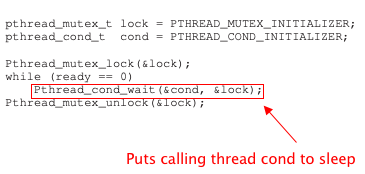
\includegraphics[width=0.7\linewidth]{../../images/midterm_2_solution_9.png}
    \end{center}

    \item \texttt{pthread\_cond\_signal}

    \begin{itemize}
        \item Is used to \underline{unblocks at least one} of the threads that
        are blocked on the specified condition variable cond
    \end{itemize}

    \bigskip

    \underline{\textbf{Example}}

    \begin{center}
    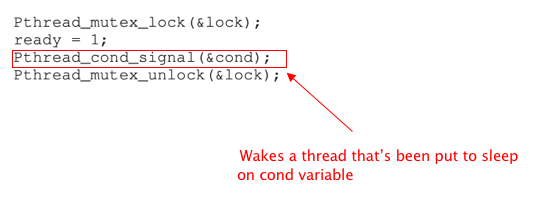
\includegraphics[width=0.8\linewidth]{../../images/midterm_2_solution_10.png}
    \end{center}

\end{itemize}

\section{Condition Variable}

\begin{itemize}
    \item is an explicit queue that threads can put themselves on when some
    state of execution is not as desired (so it can be put to sleep)
    \item when states are changed, one or more of the waiting threads can be
    awaken and be allowed to continue (done by \textbf{signaling} the condition)
    \item queue is \textbf{FIFO}
    \item \texttt{wait()} call is used to put thread to sleep
    \item \texttt{singal()} call is used to awake thread from sleep
    \item \textbf{Syntax (initialization):}

    \bigskip

    \texttt{pthread\_cont\_t c = PTHREAD\_COND\_INITIALIZER}

    \bigskip

    \underline{\textbf{Example}}

    \begin{center}
    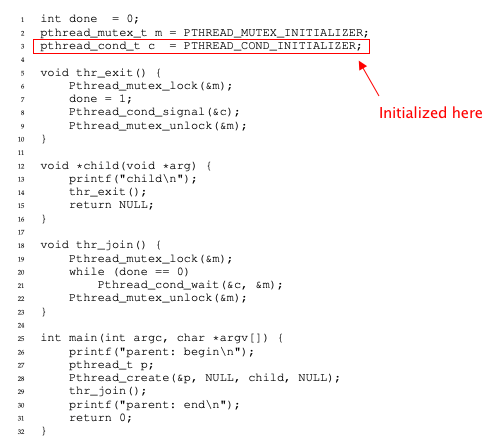
\includegraphics[width=\linewidth]{../../images/midterm_2_solution_16.png}
    \end{center}

    \item

    \textbf{Syntax (Wait):}

    \bigskip

    \texttt{Pthread\_cond\_wait(pthread\_cond\_t *c, pthread\_mutex\_t *m)}

    \bigskip

    \underline{\textbf{Example}}

    \begin{center}
    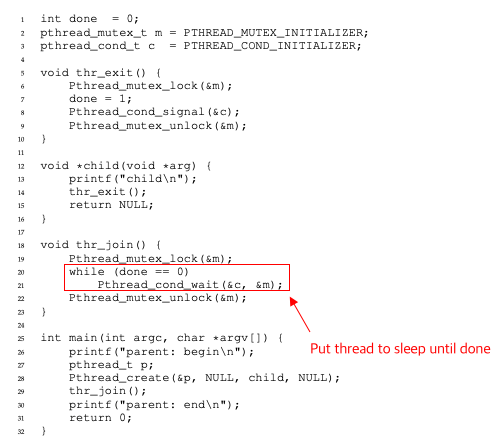
\includegraphics[width=\linewidth]{../../images/midterm_2_solution_17.png}
    \end{center}
    \item \textbf{Syntax (Signal):}

    \bigskip

    \texttt{Pthread\_cond\_signal(pthread\_cond\_t *c)}

    \underline{\textbf{Example}}

    \begin{center}
    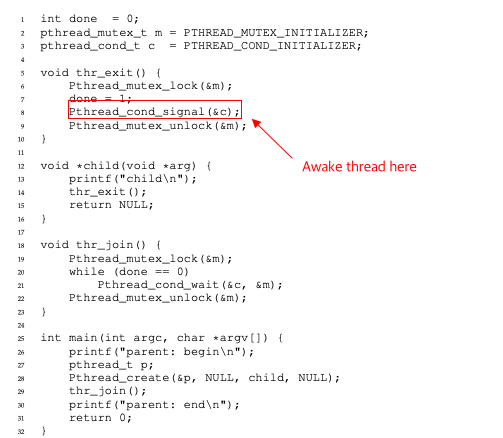
\includegraphics[width=\linewidth]{../../images/midterm_2_solution_18.png}
    \end{center}

\end{itemize}

\section{Spinlock}
\begin{itemize}
    \item Is the simplest lock to build
    \item Uses a lock variable

    \begin{itemize}
        \item 0 - (available/unlock/free)
        \item 1 - (acquired/locked/held)
    \end{itemize}

    \item Has two operations

    \begin{enumerate}[1.]
        \item \texttt{acquire()}

        \bigskip

        \begin{center}
        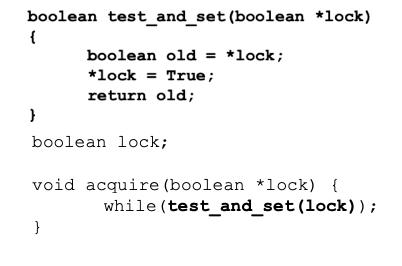
\includegraphics[width=0.7\linewidth]{../../images/midterm_2_solution_3.png}
        \end{center}

        \bigskip

        \item \texttt{release()}

        \bigskip

        \begin{center}
        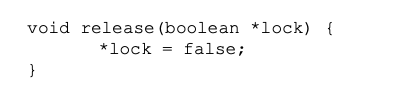
\includegraphics[width=0.7\linewidth]{../../images/midterm_2_solution_4.png}
        \end{center}

        \bigskip
    \end{enumerate}
    \item Allows a single thread to enter critical section at a time
    \item Spins using CPU cycles until the lock becomes available.
    \item May spin forever
\end{itemize}

\section{Livelock}

\begin{itemize}
    \item Two or more threads reapeatedly attempting this code over and over (e.g acquiring lock), but progress is
    not being made (e.g acquiring lock)
    \item Solution: Add a random delay before trying again (decrease odd of livelock)
\end{itemize}

\section{Mutual Exclusion}

\begin{itemize}
    \item Is a guarentee that is one thread is executing within the critical section,
    the others will be prevented from doing so.
\end{itemize}

\section{Deadlock}

\begin{center}
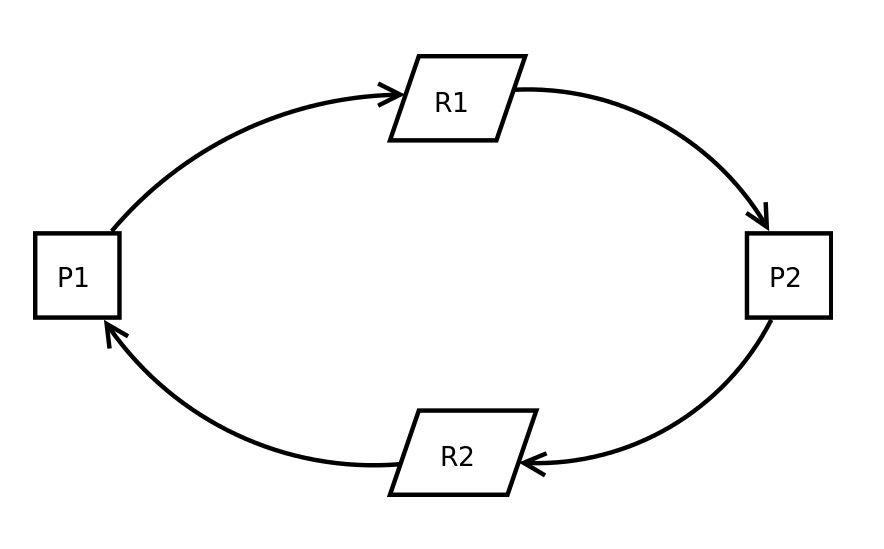
\includegraphics[width=0.6\linewidth]{../../images/midterm_2_solution_11.png}
\end{center}

\begin{itemize}
    \item Is a state in which each member of a group is waiting for
    another member including itself, to take action (e.g. releasing lock)
    \item Conditions for Deadlock (All four must be met)

    \begin{itemize}
        \item \textbf{Mutual Exclusion}
        \begin{itemize}
            \item Occurs when threads claim exclusive control of resources that
            they require (e.g. thread grabing a lock)
        \end{itemize}
        \item \textbf{Hold-and-wait}
        \begin{itemize}
            \item Occurs when threads hold resources allocated to them (e.g locks that they have already acquired)
            while waiting for additional resources (e.g. locks that they wish to acquire)
        \end{itemize}

        \item \textbf{No Preemption}
        \begin{itemize}
            \item Occurs when resource cannot be forcibly removed from threads that are holding them
        \end{itemize}
        \item \textbf{Circular Wait}
        \begin{itemize}
            \item Occurs when there exists a circular chain of threads such that
            each threads hold one or more resources (e.g. locks) that are being
            requested by the next thread in the chain.
        \end{itemize}
    \end{itemize}

    \bigskip

    \underline{\textbf{Example}}

    \begin{center}
    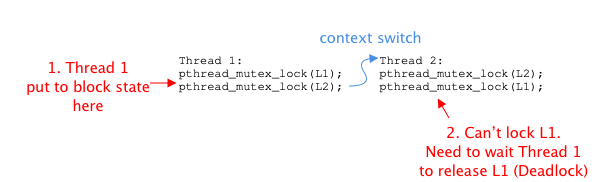
\includegraphics[width=0.9\linewidth]{../../images/midterm_2_solution_12.png}
    \end{center}

    \item Preventions

    \begin{itemize}
        \item \textbf{Circular Wait}
        \begin{itemize}
            \item Write code such that circular wait is never induced
            \item Is the most practical prevention technique
            \item Requires deep understanding of the code base
            \item \textbf{Total Ordering} (Most starightforward)

            \bigskip

            \underline{\textbf{Example}}

            \bigskip

            Given two locks in the system (\texttt{L1} and \texttt{L2}), always
            acuiqure \texttt{L1} before \texttt{L2}

            \bigskip

            \item \textbf{Partial Ordering} (Applied to complex systems)

            \bigskip

            \underline{\textbf{Example}}

            \bigskip

            Memory mapping code in Linux (has then different groups).

            \bigskip

            (Simple) \texttt{i\_mutex} before \texttt{i\_mmap\_mutex}

            \bigskip

            (More complex) \texttt{i\_mmap\_mutex} before \texttt{private\_lock}
            before \texttt{swap\_lock} before \texttt{mapping->tree\_lock}

        \end{itemize}

        \item \textbf{Hold-and-wait}
        \begin{itemize}
            \item Can be avoided by acquiring all locks at once
            \item Can be problematic
            \item Must know which lock must be held and acquire ahead of time
            \item Is likely to decrease concurrency (since all need to be acquired over their needs)

            \bigskip

            \underline{\textbf{Example}}

            \bigskip

            \begin{center}
            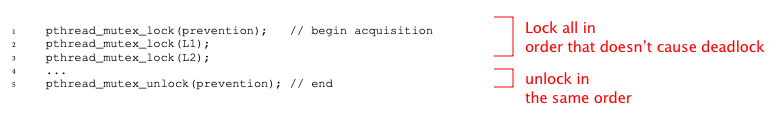
\includegraphics[width=\linewidth]{../../images/midterm_2_solution_13.png}
            \end{center}
        \end{itemize}

        \item \textbf{No Preemption}
        \begin{itemize}
            \item Can be avoided by adding code that force unlock if not available

            \begin{center}
            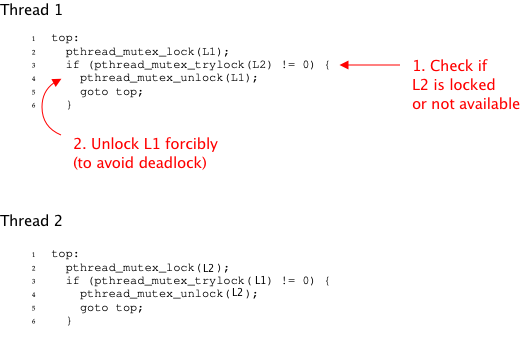
\includegraphics[width=0.8\linewidth]{../../images/midterm_2_solution_14.png}
            \end{center}

            \item \texttt{pthread\_mutex\_trylock} tries to lock the speicied mutex.
            \item \texttt{pthread\_mutex\_trylock} returns 0 if lock is available
            \item \texttt{pthread\_mutex\_trylock} returns the following error if occupied

            \bigskip

            \quad \texttt{EBUSY} - Mutex is already locked

            \bigskip

            \quad \texttt{EINVAL} - Is not initialized mutex

            \bigskip

            \quad \texttt{EFAULT} - Is in valid pointer

            \item May result in \textbf{live lock}
        \end{itemize}

        \item \textbf{Mutual Exclusion}
        \begin{itemize}
            \item Idea: Avoid the mutual exclusion at all
            \item Use \textbf{lock-free}/\textbf{wait-free} approach:
            building data structures in a manner that does not require explicit locking
            using hardware instructions

            \bigskip

            \underline{\textbf{Example}}

            \bigskip

            \begin{center}
            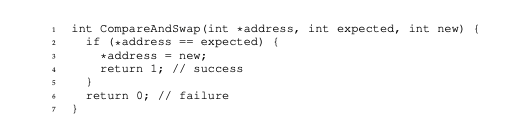
\includegraphics[width=\linewidth]{../../images/midterm_2_solution_15.png}
            \end{center}

        \end{itemize}
    \end{itemize}

    \item Avoidance

    \begin{itemize}
        \item \textbf{Banker's Algorithm}
    \end{itemize}
\end{itemize}

\section{Process}

\begin{itemize}
    \item Is a program in execution
    \item Is named by it's process ID or PID
    \item Can be described by the following states at any point in time

    \begin{itemize}
        \item Address Space
        \item CPU Registers
        \item Program Counter
        \item Stack Pointer
        \item I/O Information
    \end{itemize}

    (wait. this is PCB)

    \item Exists in one of many different \textbf{process states}, including

    \begin{enumerate}[1.]
        \item Running
        \item Ready to Run
        \item Blocked
    \end{enumerate}

    \bigskip

    \begin{itemize}
        \item Different events (Getting Scheduled, descheduled, or waiting for I/O)
        transitions one of these states to the other
    \end{itemize}

\end{itemize}

\section{Coarse-grained-locking}

\begin{itemize}
    \item Is one big lock that is used any time any critical section is accessed
    \item Is easy to write
    \item Is easy to prove correctness
    \item No fault-tolerance but deadlock-free
    \item Perfoms poorly when contention (the need for performance due to load) is high
    \begin{itemize}
        \item No concurrent access
    \end{itemize}

    \bigskip

    \underline{\textbf{Example}}

    \bigskip

    \begin{center}
    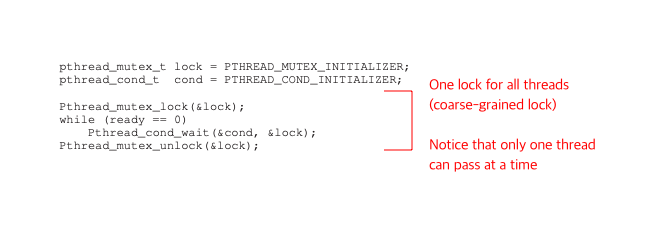
\includegraphics[width=\linewidth]{../../images/midterm_3_solution_10.png}
    \end{center}
\end{itemize}


\section{Fine-grained-locking}

\begin{itemize}
    \item Uses different locks to often protect different data and data strutures
    \item Allows more threads to be in locked code at once

    \bigskip

    \underline{\textbf{Example}}

    \bigskip

    \begin{center}
    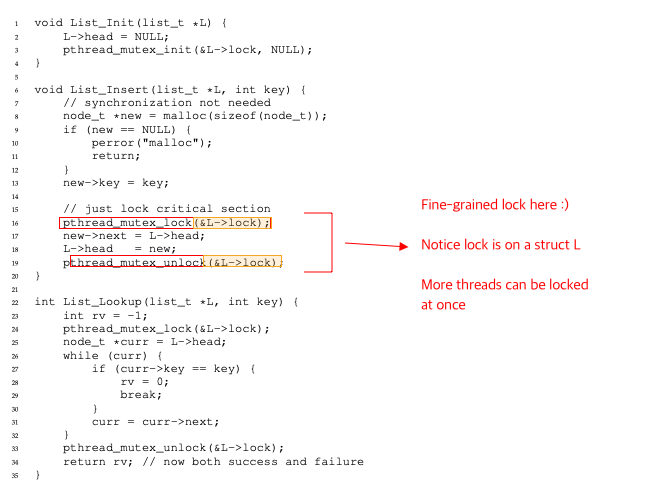
\includegraphics[width=\linewidth]{../../images/midterm_3_solution_11.png}
    \end{center}

\end{itemize}
\section{Hand-over-hand locking}

\begin{itemize}
    \item Idea: instead of having a single lock for the entire list, a lock per node
    of the list is added; when traversing the list, the list grabs the next node's lock,
    and releases the current node's lock
    \item Is a fine-grained-locking
    \item Holds at most 2 locks at a time

    \bigskip

    \underline{\textbf{Example}}

    \bigskip

    \begin{center}
    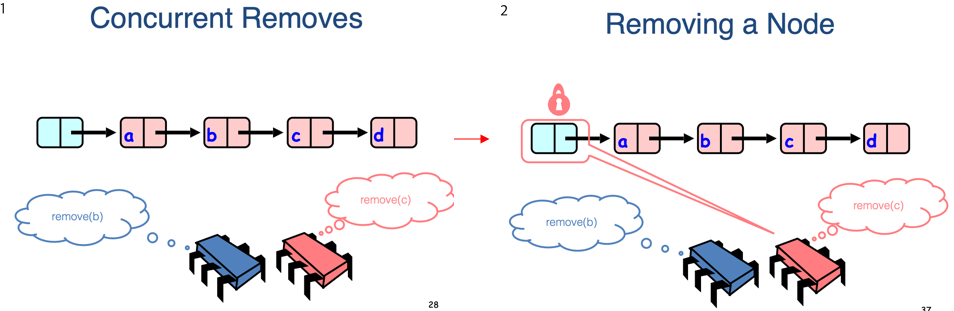
\includegraphics[width=\linewidth]{../../images/midterm_3_solution_3.png}
    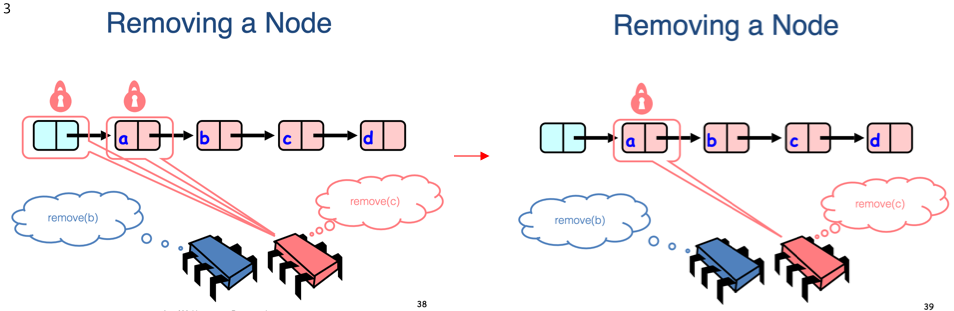
\includegraphics[width=\linewidth]{../../images/midterm_3_solution_4.png}
    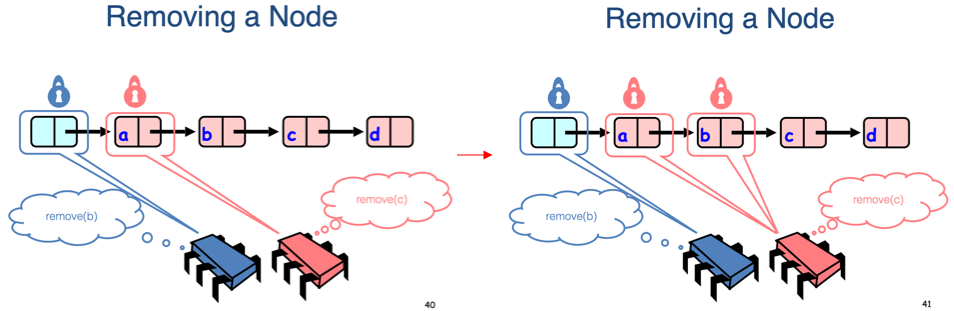
\includegraphics[width=\linewidth]{../../images/midterm_3_solution_5.png}
    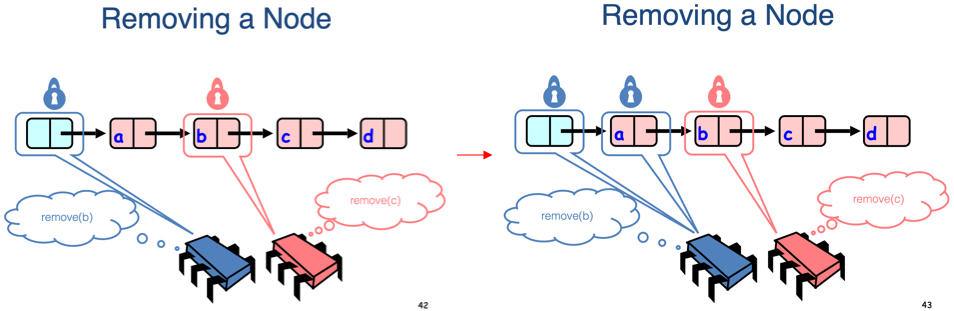
\includegraphics[width=\linewidth]{../../images/midterm_3_solution_6.png}
    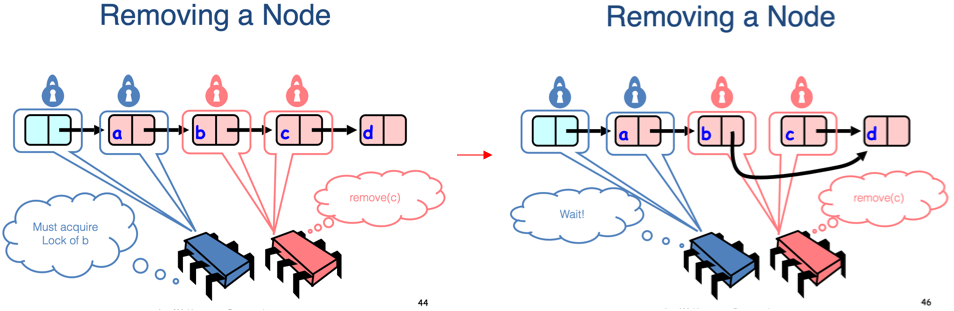
\includegraphics[width=\linewidth]{../../images/midterm_3_solution_7.png}
    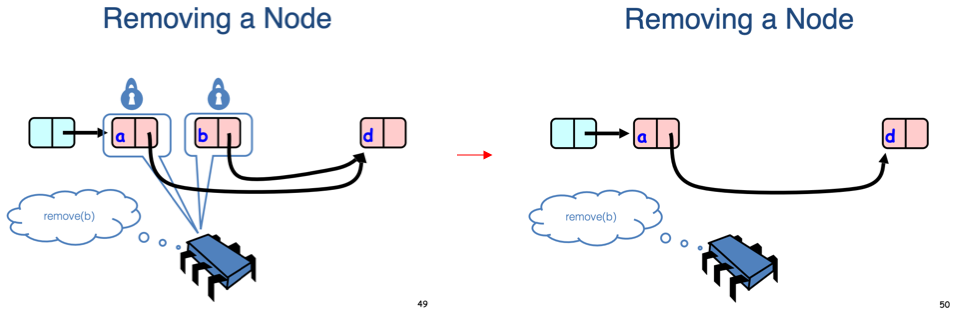
\includegraphics[width=\linewidth]{../../images/midterm_3_solution_8.png}
    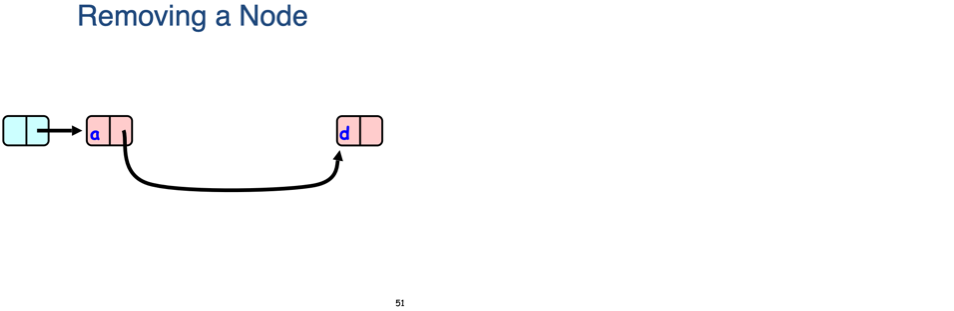
\includegraphics[width=\linewidth]{../../images/midterm_3_solution_9.png}
    \end{center}

\end{itemize}


\end{document}